\chapter{Methodology}

\section{Data Selection}
The first point for considering what dataset to use for this project was to identify a product that was open-source, and with a resolution less than one metre. It had to comprise of an RGB image with an associated mask layer representing the feature or features of interest. In Richmond (2019) Table \ref{tab.datasets}, displays all the datasets considered can be found with justifications for each. For this thesis the INRIA Building Dataset was used, this dataset was developed for the project outlined in \cite{maggiori17a}. Their dataset was created in order to ensure it contained recent orthorectified imagery; recent official cadastral records; precise registration between orthorectified imagery and cadastral records; open access data, for both imagery and cadaster; and coverage that varied across urban landscapes and illumination. \cite{maggiori17a} found that there were certain areas in Austria and the US that satisfied these requirements and they focused on zones where reference data and images were available. The US imagery was provided at either 15 or 30cm resolutions with three to four spectral bands and the Austrian data contains three bands ar a resolution of 10 or 20 cm. They built the dataset to be consistent at 30 cm and RGB by using average re-sampling where needed. For there feature mask they considered two classes, \textit{building} and \textit{not building}. Once this was done they visually inspected the imagery to ensure the cadaster datasets were properly aligned with the imagery, removing cities where irregular shifts had occurred. 

\begin{table}[htbp]
\centering
\begin{adjustbox}{width=1\textwidth,center=\textwidth}
\begin{tabular}{l|llll|ll}
\textbf{Train}      & Tiles* & Total area &  & \textbf{Test}       & Tiles* & Total area \\ \cline{1-3} \cline{5-7} 
Austin, TX          & 36     & 81 km$^2$     &  & Bellingham, WA      & 36     & 81 km$^2$     \\
Chicago, IL         & 36     & 81 km$^2$     &  & San Francisco, CA   & 36     & 81 km$^2$     \\
Kitsap County, WA   & 36     & 81 km$^2$     &  & Bloomington, IN     & 36     & 81 km$^2$     \\
Vienna, Austria     & 36     & 81 km$^2$     &  & Innsbruck, Austria  & 36     & 81 km$^2$     \\
West Tyrol. Austria & 36     & 81 km$^2$     &  & East Tyrol, Austria & 36     & 81 km$^2$     \\
Total               & 180    & 405 km$^2$    &  & Total               & 180    & 405 km$^2$   
\end{tabular}
\end{adjustbox}
\caption[Dataset statistics.]{Dataset statistics. *Tile size:1500$^2$ px. (0.3m resolutions) taken from \cite{maggiori17a}.}
\label{tab.inria_dataset}
\end{table}

Table \ref{tab.inria_dataset} depicts the regions the regions included in the datasets and their distribution between training and test subsets. The dataset was split in evenly between training and test in order to allow for a proper assessment of the methods and how they can generalise to other areas. It was also split to ensure that each subset contained American and European examples as well as high-density urban areas (Chicago/San Francisco and Vienna/Innsbruck) and low-density (Kitsap/Bloomington and West/East Tyrol). \cite{maggiori17a} even made sure that some of the groups contained dissimilar information (e.g. the image from Kitsap County were taken from different flights with different characteristics). They created the reference data by rasterizing the cadastral shapefiles using GDAL and examples can be found in Figure \ref{fig.inria_dataset}.

\begin{figure}[htpb]
    \centering
    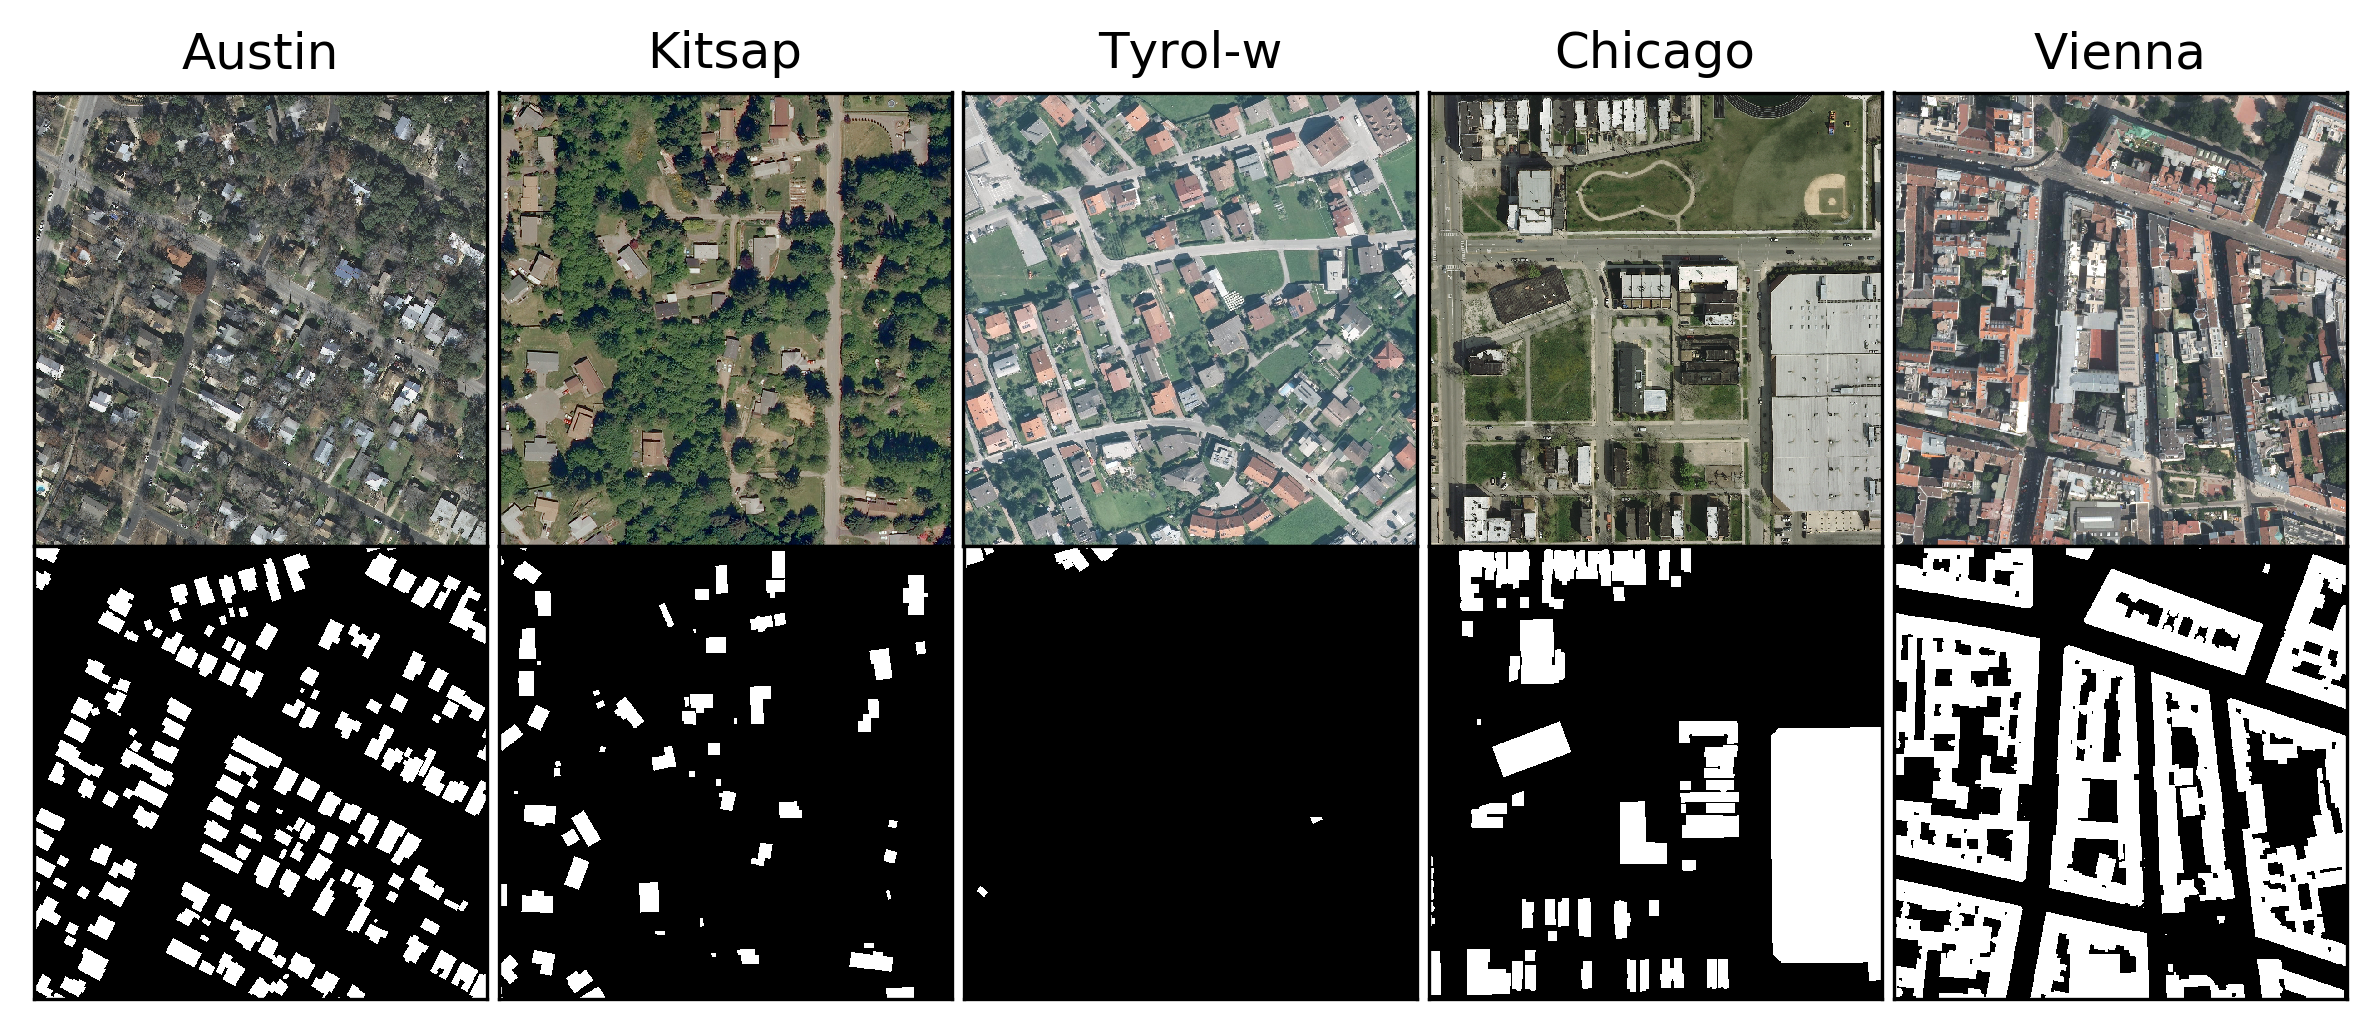
\includegraphics[width=1\textwidth]{\dir/figs/example_inria.png}
    \caption[Examples from the INRIA Image Labelling Dataset]{Example of individual tiles from the train dataset and their corresponding reference data. Images show the full extent of the tiles, 5000px.}
    \label{fig.inria_dataset}
\end{figure}



\section{Model Architecture}
For a more detailed discussion of how CNNs work refer to Richmond (2019), this section will discuss the architecture of the CNN and justify why certain elements were chosen over others. 
\section{Performance}

\section{Hyperparameter Tuning}

